% options:
% thesis=B bachelor's thesis
% thesis=M master's thesis
% czech thesis in Czech language
% english thesis in English language
% hidelinks remove colour boxes around hyperlinks

\documentclass[thesis=B,czech]{FITthesis}[2012/06/26]

\usepackage[utf8]{inputenc} % LaTeX source encoded as UTF-8

\usepackage{graphicx} %graphics files inclusion
\usepackage{amsmath} %advanced maths
% \usepackage{amssymb} %additional math symbols

\usepackage{dirtree} %directory tree visualisation
%\usepackage{color}
% % list of acronyms
% \usepackage[acronym,nonumberlist,toc,numberedsection=autolabel]{glossaries}
% \iflanguage{czech}{\renewcommand*{\acronymname}{Seznam pou{\v z}it{\' y}ch zkratek}}{}
% \makeglossaries

\newcommand{\tg}{\mathop{\mathrm{tg}}} %cesky tangens
\newcommand{\cotg}{\mathop{\mathrm{cotg}}} %cesky cotangens
\newcommand{\TODO}[1]{\textbf{\textsc{TODO:} #1}}

% % % % % % % % % % % % % % % % % % % % % % % % % % % % % % 
% ODTUD DAL VSE ZMENTE
% % % % % % % % % % % % % % % % % % % % % % % % % % % % % % 

\department{Katedra teoretické informatiky}
\title{Minimalizace výškového převýšení při vyhledávání trasy v~mapě}
\authorGN{Pavel} %(křestní) jméno (jména) autora
\authorFN{Zbytovský} %příjmení autora
\authorWithDegrees{Pavel Zbytovský} %jméno autora včetně současných akademických titulů
\supervisor{Ing. Jitka Hrabáková}
\acknowledgements{Na tomto místě bych rád poděkoval vedoucí práce Ing. Jitce Hrabákové za její velikou pomoc, podnětné rady a vstřícnost. Za podporu děkuji rodině a blízkým. Za rady k~sazbě textu Jakubovi Luckému.}

\abstractCS{
Tato práce se zabývá minimalizací převýšení při vyhledávání cyklistické trasy v~mapě, které je identifikováno jako zásadní rozdíl mezi cyklistickou a ostatní dopravou. V~první části jsou rozebrány dostupné routovací systémy a povaha otevřených mapových dat. Výsledkem celé práce je implementace navrženého modelu cyklisty do systému Routino. K~dosažení tohoto modelu je využito analyzátoru zaznamenaných tras z~GPS a digitálních modelů zemského povrchu, které jsou důkladně popsány.
}

\abstractEN{
This bachelor's thesis focuses on elevation minimization for bicycle routing, which is identified as a main difference among other types of transport. First part consists of comparison of availible routing systems, as well as nature of open map data. As the result the designed cyclist's model is implemented in the Routino routing system. This result makes use of GPS traces analyzer and digital elevation models, which are covered thorougly.
}

\placeForDeclarationOfAuthenticity{V~Praze}
\declarationOfAuthenticityOption{1} %volba Prohlášení
\keywordsCS{routování cyklistů, minimalizace převýšení, OpenStreetMap, SRTM}
\keywordsEN{routing for cyclists, elevation minimization, OpenStreetMap, SRTM}

\usepackage{graphicx}
\usepackage{amsmath}
\begin{document}

% \newacronym{CVUT}{{\v C}VUT}{{\v C}esk{\' e} vysok{\' e} u{\v c}en{\' i} technick{\' e} v Praze}
% \newacronym{FIT}{FIT}{Fakulta informa{\v c}n{\' i}ch technologi{\' i}}


\begin{introduction}

Tématem této bakalářské práce je \uv{minimalizace výškového převýšení při vyhledávání trasy v~mapě}. Vyhledávání tras je dnes velice užitečným nástrojem pro cyklisty i automobilisty. Nejčastější použití vidíme v~embedded zařízeních jako navigace či chytré telefony, které se vyznačují algoritmy úspornými na paměť i výpočetní výkon. Druhým rozšířeným případem je pak serverové řešení, které uživatelé znají v~podobě online webových \mbox{aplikací}.

Tato práce se zaměřuje na serverové řešení pro cyklisty a vychází z~vlastní zkušenosti, že dostupné online plánovače nezohledňují převýšení. Optimalizace převýšení by mohla být možná oběma směry – jednak nabídnout k~nejkratší trase alternativu s~optimalizovanou výškou, a dále také umožnit zajímavou objížďku s~větším převýšením. Zde se ale budeme věnovat především minimalizaci, neboť ta je cyklisty více žádána.

Samotné plánování trasy je pro cyklisty přínosem především při používání kola jako dopravního prostředku. Při cestování skrz město nebo neznámou krajinou je velmi často nějaký druh navigace potřeba. Turistické využití plánovačů je menší, neboť tyto uživatele zajímá spíše jedna značená cyklotrasa či používají připravené tištěné průvodce.

V~současnosti je v~oblasti plánovaní tras pro cyklisty ještě stále co zlepšovat. Kromě nastavení jednoho správného modelu je možné též nabídnout uživateli analýzu jeho projetých tras a tedy přizpůsobit výsledky přímo pro~něj.

Zdá se, že v~budoucnosti bude narůstat míra využití otevřených mapových dat a právě projekt OpenStreetMap může hrát velikou roli i v~Čechách. 

V~první kapitole se podíváme na základní pojmy routování a důkladně porovnáme dostupné systémy k~možné úpravě.

V~druhé kapitole se zaměřujeme již na optimalizaci převýšení, vysvětlíme, proč není žádoucí úplná minimalizace a připravíme též nástroj na analýzu projetých tras, který využijeme pro přípravu modelu cyklisty.

Ve třetí, implementační, kapitole navrhneme úpravy zvoleného routovacího systému a doplníme jej o~načítání výškového modelu.

Poslední kapitola komentuje výstupy této práce, tedy ukázky nalezených tras. Porovnáme dosažené výsledky s dostupnými systémy, včetně těch, které se již optimalizaci převýšení věnují.



\end{introduction}


























% 1.--------------------------------------------------------------
% --------------------------------------------------------------
\chapter{Používané routovací systémy}
% --------------------------------------------------------------
% --------------------------------------------------------------
Routovací systém má za úkol nalézt a vrátit trasu mezi dvěma body na reálných datech, skládá se samozřejmě z~několika částí. Asi největší význam má samotný vyhledávací algoritmus, který se snaží minimalizovat určenou podmínku, například minimalizujeme vzdálenost či výsledný čas. Další leč opomíjenou části jsou mapová data. Sice se nejedná o~informatickou zdatnost, ale i zde bychom se bez informačních technologií neobešli. 


% 1.1 --------------------------------------------------------------
% --------------------------------------------------------------
\section{Mapová data}
% --------------------------------------------------------------
% --------------------------------------------------------------

Je zřejmé, že kvalita dat má zásadní dopad na výsledky routovacího systému. Prvotním požadavkem je samozřejmě hustota dat a tedy co největší podobnost s~reálnou průchodností silniční, cyklistické či pěší sítě. Ovšem ještě zásadnější je informatická užitnost - vektorový zápis dat a topologická návaznost, požadavek tedy je, aby vstupními daty byl obecný graf $G = <V,E>$, kde $V$ je množina vrcholů, typicky se zeměpisnou délkou a šířkou a $E$ je množina hran, tedy $ E \subseteq V \times V $. 

S~těmito daty už můžeme minimalizovat vzdálenost, ale pro routování zpravidla potřebujeme ještě jeden parametr a to nějaký způsob popisu hran. Typicky se bude jednat o~popis typu komunikace (např. dálnice, klasifikovaná silnice, vozová cesta, lesní pěšina, či třeba informace zdali se jedná o~značenou cyklotrasu). Můžeme si tedy rozšířit definici hrany na $E \subseteq V \times V \times T$, kde $T$ je množina vlastností.

Získání dat není jednoduchá záležitost, k~dispozici jsou jednak komereční datasety, které pro studentské použití zpravidla půjčují nějaké části  - např. společnost GeoDIS, či CENIA. Dále ke slovu přichází různé opensource projekty, napřiklad mapovou wikipedii provozují Wikimapia.org, OpenStreet-Map.org či crowdsourcovanou autonavigaci služba Waze.

Z~tohoto množství geodat jsou zcela nevhodná rastrová dat, neboť z~nich nelze jednoduše získat routovatelný graf, dále ty jež neobsahují topologickou informaci (např. Wikimapia.org) a též všechny, které se specializují pouze na automobilový segment (Waze, ŘSD). Zbývá nám tedy služba OpenStreetMap.

OpenStreetMap je mapová databáze, kterou může každý editovat a k~vektorovým datům přidávat zcela libovolné vlastnosti. Ovšem aby data měla nějakou užitnou hodnotu, tak komunita zajišťuje dohodu, jaké vlastnosti budou popisovat konkrétní reálné objekty. Vznik celého datasetu je založen na dobrovolnické práci, jednak importy z~dostupných Public Domain zdrojů (napr. úřední dílo), dále obkreslování cest a jiných objektů z~Public Domain leteckých snímků. A~v~neposlední řadě reálné procházení terénu s~GPS a následné vložení do mapy spolu s~přidanými informacemi.

Díky komunitní shodě má takováto mapa velkou výhodu, kterou je konzistetní používání vlastností napříč celým světem, ovšem na snadě je i nevýhoda. Kvalita dat je závislá na koncentraci přispěvatelů v~daném místě, snadno se tak může stát, že někde třeba chybí silnice či celé město. Naopak v~místech s~větší popularitou mapové podklady převyšují v~množství detailů i dostupné komereční podklady. V~ČR je situace převážně velice dobrá a vývin počtu přispěvatelů také příznivý.


% 1.2--------------------------------------------------------------
% --------------------------------------------------------------
\section{Minimalizační podmínka -- jádro routování} 
\label{minimalizacniPodminka}
% --------------------------------------------------------------
% --------------------------------------------------------------


Nyní se dostáváme ke hlavní tezi této práce. Jak již bylo naznačeno, je snadno možné minimalizovat vzdálenost. S~časem je to o~něco těžší - musíme odhadnout rychlosti na různých typech cest a dle toho spočítat teoretický čas, který můžeme též minimalizovat. Oba tyto modely velice dobře fungují pro automobilovou i pěší dopravu, ovšem právě onu výjimku tvoří cyklisté.

\emph{Cyklistův čas není ani tak ovlivněn typem komunikace, jako především nastoupaným převýšením.} Uvědomme si, že automobily překonávají kopce bez zpomalení a stejně tak i u~pěších se rychlost skoro nemění. Většina dostupných routerů se primárně specializuje na auta a cyklisty mají jako přidanou hodnotu. Ovšem algoritmy jsou využity stejné, a tak hledání nejkratší trasy kopce vůbec nezohledňuje.

Samotné srovnání dostupných routerů je v~podkapitole \ref{porovnaniSystemu}. Také nesmíme zapomenout, že používání stejného modelu pro auta i pro cyklisty může dávat naprosto správné výsledky, pokud je oblast plochá či mírně zvlněná a především neobsahuje samostatné kopce, které lze objet. Například v~Holandsku či pobřeží USA tak celá naše myšlenka ztrácí smyl. Ovšem zdá se, že v~České republice by mohla hrát velkou roli.

Cílem této práce je právě zohlednit kopce při routování cyklotrasy, uvidíme, zda je tato snaha užitečná a jestli to při kopcovitosti naší země opravdu hraje nějakou roli.

% 1.3 --------------------------------------------------------------
% --------------------------------------------------------------
\section{Porovnání routovacích systémů}
\label{porovnaniSystemu}
% --------------------------------------------------------------
% --------------------------------------------------------------
V~současnosti existuje veliké množství online vyhledávačů tras, v~podstatě každý mapový server má své vlastní řešení. Ovšem jen některé umožňují vyhledávat cyklotrasy. Open-source systémů nad OpenStreetMap daty najdeme též desítky, většinou se jedná o~navigační zařízení pro mobilní telefony a smartphony. Ovšem těch, které plánují pro cyklisty a zároveň jsou určeny pro webový serverový provoz, už je jen několik. Dva z~nich se dokonce zaměřují na cyklisty a umí i zohledňovat kopce, bohužel tyto nejsou open-source a tak nelze zjistit jaké algoritmy využívají, můžeme je ale využít pro porovnání výsledků.

Základní srovnání systémů je v~tabulce \ref{table:srovnani} (částečně převzato z~\cite{osmwiki-routers}). Nyní se podívejme na zmíněné systémy podrobněji.


\begin{table}[h!]
\begin{tabular}{l|l|l|l} %poslední {} v tomto řádku formátuje tabulku
\textbf{název} & \textbf{open source} & \textbf{jazyk} & \textbf{cyklo-routování}  \\
\hline
OpenRouteService   & ne   & Java   & ano    \\
YOURS / Gosmore    & ano, BSD & Java / C++ & ano \\
CycleStreets       & ne (zatím) & PHP & ano, i kopce \\
Cloudmade & ne & -- & ano \\
MapQuest & ne &  -- & ano \\
Routino  &  ano, AGPL &  C & ano \\
BBBike & ano, GPL& Perl/Tk& ano \\
OSRM  &  ano, AGPL & C++ / Boost & ne \\
BRouter & ne & -- & ano, i kopce
\end{tabular}
\caption{Porovnání online routovacích systémů nad OSM daty.}
\label{table:srovnani}
\end{table}



\subsection{OpenRouteService}
Tento systém nabízí pro cyklisty nejkratší trasu, trasu pro horské či silniční kolo, \uv{bezpečnou trasu} a v~beta verzi též preferenci cyklotras, podrobnosti k~nalezení v~\cite{openrouteservice}. Vyvíjí ho fakulta geoinformatiky na University of Heidelberg. Ovšem velikou překážkou jsou neveřejné zdrojové kódy, které by bylo možné získat pouze přímo komunikací s~autory a zřejmě po nastavení licenčních podmínek.

Podle informací na webových stránkách projektu je využito Javovské knihovny GeoTools (LGPL licence). Ta je zaměřena především na zobrazování vektorových mapových podkladů pro desktopové aplikace, ovšem obsahuje i modul na grafové algoritmy, konkrétně Dijkstrův algoritmus, definován v článku~\cite{dijkstra}. 

Pro tuto práci není GeoTools příliš vhodný, sice umí základní operace, ale routování cyklistů, načítání a přechování rozsáhlého grafu a zprovoznění webové služby jsou všechno problémy, které by bylo nutno vyřešit.

%http://www.openrouteservice.org/contact.php

\subsection{YOURS / Gosmore}
Tento systém, podrobněji v~\cite{yours}, je jakýmsi konglomerátem několika open-source projektů. Pro tuto práci jde především o~routovací komponentu -- jedná se o~samostatný software Gosmore. Tento software je vlastně plnohodnotná navigace pro mobilní počítače, tedy umí data vyhledávat, vykreslovat i routovat. Je možné ho ale spustit z~příkazové řádky a pro cyklisty je zde připraveno vyhledání nejkratší/nejrychlejší trasy s~možností preference cyklotras. 

Gosmore, detailně v~\cite{gosmore}, je napsán v~jazyce C++ a zobrazovací systém v~Javě. Kód je kompatibilní s~mnoha mobilními platformami, a tedy protkán jednak podmíněnými bloky pro kompilátor a jednak též příkazy souvisejícími s~grafickým výstupem. Dokumentace v~kódu je spíše sporadická, nějaký obecný manuál chybí zcela. Pro tuto práci je ovšem tento systém použitelný.

\subsection{CycleStreets}
CycleStreets (podrobnosti v \cite{cyclestreets}) je čistě webová služba fungující nad uzemím Britských ostrovů. Vzhledem ke své specializaci na cyklisty dokonce zohledňuje při navigaci kopce. Ačkoliv se záměrem autorů je otevření jejich zdrojového kódu (jak uvádí ve svém článku \cite{cyclestreets-article}), tak bohužel v~době psaní této práce stále nejsou k~dispozici. 

\subsection{Cloudmade / MapQuest}
Oba tyto názvy jsou ve skutečnosti názvy společností, které se rozhodly podporovat a využívat OpenStreetMap data. Routování nabízí pouze v~podobě webových API, a proto se ani nelze dostat ke zdrojovým kódům. Obě API však umožňují vyhledávání cyklistických tras a tak je bude možno alespoň porovnat s~našimi výstupy. Webové služby jsou dostupné na \cite{cloudmade,mapquest}


\subsection{Routino}
Routino je open-source software přímo určený pro online routovací službu. Umožňuje vyhledávaní tras pro cyklisty, ovšem neumí zřejmě preferovat cyklotrasy. Spouští se z~příkazové řádky (při online režimu jako CGI služba) a příjemnou funkcí je též možnost při vstupu nastavit váhy pro routovací algoritmus. Web projektu se nalézá na \cite{routino}, obsahuje také online routovací službu omezenou na datovou oblast Britských ostrovů.

Zdrojový kód je napsán v~čistém jazyce C pod licencí AGPL a je velmi důkladně okomentován. K~projektu je též k~dispozici dokumentace instalace, hlavního algoritmu, datových struktur, nastavení routeru apod. Routino je vhodné pro využití v~této práci.

\subsection{BBBike}
BBBike je specializovaný router pro cyklisty. Původně byl postaven jako desktopová aplikace se zobrazením mapy, nyní sice nabízí i online routování, ale je omezené kvůli efektivitě pouze na velká Evropská města. V~dokumentaci se sice mluví o~optimalizaci převýšení, ovšem webová služba tuto vlastnost nevykazuje. Rozcestník k~dokumentaci se nalézá na \cite{bbbike}.

Projekt by zřejmě šel použít pro tuto práci, ovšem dokumentace převážně chybí a část je v~německém jazyce. Též repozitář se zdrojovými daty je velice chaotický a obsahuje i nesouvisející programy.

\subsection{OSRM}
Open Source Routing Machine, podrobnosti v \cite{osrm}, je vysoce výkonnostní implementace routovacího algoritmu. Kolegové z~neměcké univerzity Karlsruhe Institute of Technology se zaměřili především na tzv. speed-up techinky \cite{osrm-article}, které zajišťují vysokou rychlost, překonovající i komereční routovací služby.

Jako jediný zatím nenabízí zcela funkční hledání cyklotras, nicméně díky velkému potenciálu by bylo zajímavé tento projekt o~cyklistickou část rozšířit. Dokumentace zdrojového kódu je velice dobrá, též je k~dispozici online wiki s~dokumentací důležitých částí programu.

Zdrojový kód je v~jazyce C++ pod licencí AGPL, založen je na knihovnách Boost. Zpracování dat je přes vnitřní LUA script. Pro tuto práci se zdá tento systém vhodný.

\subsection{BRouter}
BRouter (podrobnosti v \cite{brouter}) je další specializovaný router pro cyklisty. Klade si za cíl umožnit navigaci cyklistům se všemi náležitostmi. Jako jeden z~mála opravdu obsahuje fungující optimalizaci převýšení. Online služba je pouze na ukázku schopností, hlavní použití leží v~offline routování jako doplňková aplikace v~OS Android.

Zdrojové kódy nejsou k~dispozici a též ani mnoho informací k~projektu.

\subsection{Shrnutí}
Pro tuto práci je zásadní především možnost rozšiřitelnosti kódu, tedy úprava minimalizační podmínky. Pro optimalizaci převýšení je nutné jednak upravit samotný algoritmus a také vytvořit způsob jak získávat, ukládat a využívat výšková data. Z~těchto důvodů nelze využít systémy s~uzavřenými zdrojovými kódy, a tedy ani čisté online API. Mezi open-source kandidáty tak zůstaly projekty Gosmore, Routino, BBBike a OSRM.

Vzhledem k~tomu, že těžištěm této práce je samotná optimalizace převýšení, nejlepší je vybrat systém, který se bude nejlépe upravovat. Z~tohoto porovnání vystupují rovnocenně Routino a OSRM díky čistě serverovému použití a výborné dokumentaci. Ovšem projekt Routino již umí běžným způsobem routovat cyklistické trasy, proto se příkláním k~jeho použití.




























% 2.--------------------------------------------------------------
% --------------------------------------------------------------
\chapter{Routování s~optimalizací převýšení}
\label{routovani}
% --------------------------------------------------------------
% --------------------------------------------------------------

Ikdyž mluvíme o~optimalizaci převýšení, ve skutečnosti stále řešíme minimalizační problém vzdálenosti. Důvodem je samotné hledání trasy. Vezměme například množinu všech existujících tras mezi dvěma body, následně každé trase přiřadíme určité ohodnocení dle jejího převýšení. Z~této množiny poté můžeme vybrat trasu s~minimálním převýšením, ovšem nevíme nic o~její délce a tak může být pro praktické použítí zcela nevhodná (například může kopírovat pobřeží či říční soustavu).

Optimalizací převýšení tedy rozumíme hledání nejkratší trasy s~jistou penalizací stoupajících hran. Nyní tedy stojíme před problémem, jakou měrou hrany penalizovat. Bohužel přímou penalizaci délky hran nelze nijak dobře odhadnout, pojďme se nyní podívat na jinou možnost.

% 2.1--------------------------------------------------------------
% --------------------------------------------------------------
\section{Minimalizace času} \label{minimalizace-casu}
% --------------------------------------------------------------
% --------------------------------------------------------------
Častým požadavkem routovacích systémů není jen nejkratší cesta mezi dvěma body, ale snaha o~nejkratší dojezdový čas. Mezi vzdáleností a časovou délkou trasy platí přímá úměra, a tak stačí nalézt jen ty správné koeficienty pro jednotlivé typy silnic. Pro automobily se často používá maximální rychlost komunikací. Ohodnocení hrany tak může být jednoduchý vzorec $t=s / v$. 

Při tomto řešení vzniká už jednodušší otázka, a to jak nastavit rychlostní proměnné pro cyklistu na různých kopcích. Toto je také v~souladu s~tezí kapitoly \ref{minimalizacniPodminka}, a to že cyklistův dojezdový čas je především ovlivněn nastoupaným převýšením.

% --------------------------------------------------------------
% --------------------------------------------------------------
\section{Nástroj na rychlostní analýzu záznamů tras}
% --------------------------------------------------------------
% --------------------------------------------------------------
Myšlenka je jednoduchá, záznamy projetých tras obsahují sekvenci zaznamenaných bodů spolu s~časem, polohou a výškopisem. Kdybychom dokázali ze zaznamenaných dat vyextrahovat všechny projeté kopce a u~každého vyjádřit procentuální stoupání a průměrnou rychlost, mohli bychom dostat velmi dobré proměnné pro reálný časový model. Samozřejmě tento přístup má mnohá úskalí. 

%2.2.1
\subsection{Záznam trasy}
\label{zaznamTrasy}
Záznamy tras je nejjednodušší pořídit pomocí přístroje GPS, který je ze své podstaty nepřesný. Polohopis má odchylku průměrně 5~m, výškopis průměrně 20~m. Zaznamenané body jsou ukládány po několika vteřinách, na rovnějších úsecích potom po delší době. 

Samotný systém GPS funguje na bázi triangulace polohy alespoň tří družic, které vysílají mikrovlnný signál nesoucí přesný atomový čas. Primárním problémem je tedy přímá viditelnost z~GPS zařízení na ony družice. Nejmarkantnější je situace například u~skalní stěny či mezi budovami, kde typicky jedna z~družic nemá přímou viditelnost, a navíc díky odrazům se jiné družice mohou jevit na jejím místě. Druhým významným rušením jsou přírodní tlumiče - lesní porost a oblačnost. Zde sice viditelnost zůstává zachována, ale mikrovlnný signál je přes tyto překážky mírně zpomalen a tak se může družice jevit dál. Nepřesnost může být cca 20~m, u~homogenního tlumení nebude tak výrazná.

Uvnitř budovy samozřejmě takový systém fungovat nebude. Většinu signálů vyhodnotí zařízení jako vadné, některé spočítá s~výraznou odchylkou -- dle viditelnosti až stovky metrů. Výřez na obrázku \ref{img:gpsSkakani}. Nenechme se zmást automobilovou navigací, která \uv{umí} navigovat i v~tunelech, ve většině případů se jedná o~simulaci, někdy korigovanou daty z~akcelerometru.

Je tedy třeba mít na paměti, že GPS je nepřesný zdroj, ovšem mimo popsané situace vykazuje velmi dobré výsledky. Jiné možnosti se bohužel nenabízí. Pro armádní a geodetické účely existuje ještě tzv. kódovaná GPS, která má přesnost v~řádu centimetrů, pro naše použití je ale cenově nedostupná. Geoinerciální systémy jsou zatím na začátku vývoje a zásadním problémem je narůstající zkreslení s~časem.


 \begin{figure}\centering
 	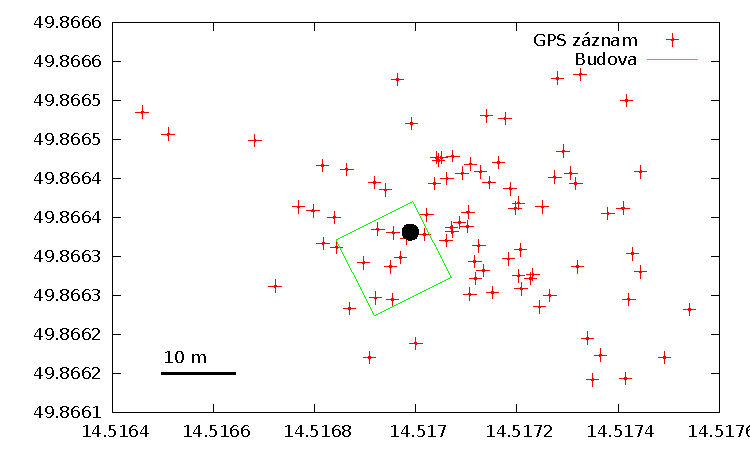
\includegraphics{grafy/gps.pdf}
 	\caption{Ukázka nepřesnosti záznamu uvnitř budovy. Černý bod označuje polohu dle mapy.}
	\label{img:gpsSkakani}
 \end{figure}



%2.2.2
\subsection{Digitální výškový model Země}
\label{dem}
Abychom zpřesnili výškopis u~záznamu trasy máme možnost využít digitálního modelu naší planety  (anglicky DEM - Digital Elevation Model). Ten vzniká většinou satelitním nebo leteckým snímkování území, výstupem pak je čtvercová souřadnicová síť, kde na každém průsečíku je vynesena výška. 

Výhodou takového modelu pro účely analýzy tras je především imunita vůči rušení signálu, na druhou stranu velkou nevýhodou je malé rozlišení (cca 50 m) a s~tím spojená nutnost interpolovat prostory mezi průsečíky. Výraznější ovlivnění je u~prudkých srázů a skalních stěn, kde je skokovitá změna rozmělněna do celého interpolovaného prostoru. Ačkoliv tedy zaznamený bod může ležet na rovné ploše pod kolmým útvarem, v~digitálním modelu se nám zobrazí třeba uprostřed.

Pro naši práci hledáme volně použitelný zdroj:
\begin{itemize}
\item{SRTM DEM - Výškový model nasnímala NASA v~roce 2000. Původní rozlišení 1 úhlová vteřina zeměpisné délky a šířky, odtud název SRTM1. V~jednom úhlovém stupni tedy $3600 \times 3600$ bodů, což dává v~našich polohách rozlišení asi 30 m. Licence Public Domain.

Protože SRTM1 data vykazovala velké množství šumu, používá se nyní zprůměrovaní hodnot z~$3 \times 3$ úhlových vteřin, odtud označení SRTM3. Podrobnosti v  \cite{dem-srtm}. Druhým problémem SRTM dat jsou nezměřené body tzv. díry (voids) - abychom na tato data nenarazili je možné využít interpolací zaplněnou verzi od CGIAR konzorcia, tzv. SRTM3 verze~4. Podrobnosti v \cite{dem-srtm-cgiar}.
}

\item{ASTER GDEM - V~roce 2009 proběhlo nové satelitní snímkování ve spolupráci japonských úřadů a NASA. Tento dataset má opět rozlišení 1 úhlové vteřiny a o~mnoho větší pokrytí, ovšem díky výskytu artefaktů a celkově probíhajícím pracem je zatím označen jako “dílo ve výzkumu” a není doporučen k~běžnému použití. Licence je volná pro nekomereční použití. Podrobnosti v \cite{dem-aster}.}

\item{Google Elevation API - Samotné použití webového API pro analýzu tras je docela dobře možné. Měření výšky je totiž nutno provést u~realtivně malého počtu bodů (řádově stovky za hodinu záznamu). Zásadnějším problémem je zde licence, která povoluje využití API pouze pro zobrazení nad mapovými podklady Google Maps. Podrobnosti v \cite{dem-google}.}
\end{itemize}

Z~těchto informací tedy vyplývá jako nejvhodnější použití ASTER GDEM modelu, ovšem dle zadání se budeme držet SRTM a ASTER zkusíme využít jako referenční model.

%2.2.3
\subsection{Seskupování intervalů} 
\label{seskupovani}
Nyní se už můžeme podívat na samotný analyzátor. Z~hlediska rychlého vývoje a snadné vizualizace byly zvoleny webové technologie PHP a JavaScript. Trasové záznamy pak načítáme ve XML formátu GPX.


Jak už bylo zmíněno, záznamy tras obsahují mnoho bodů v~zatáčkách, a minimum v~rovných úsecích. Abychom tato data sjednotili, bylo třeba zvolit vhodný časový úsek a kratší intervaly do něj seskupit. Tento přístup nám umožnil sledovat výškovou změnu, která by se jinak neprojevila. Jako vhodný interval se ukázala 1 minuta, cyklista ujede cca 300 m, což vhodně převyšuje rozlišovací schopnost SRTM3 dat.

Cílem této agregace bylo především spojit krátké úseky v~delší, proto byl zvolený interval použitý jako minimální. V~případě, že původní interval je delší, je ponechán beze změny. 

%2.2.4
\subsection{Interpolace výškových dat}
K~samotnému čtení SRTM dat jsem použil PHP knihovnu od Boba Osoly, kterou zveřejnil na svém webu \href{http://www.osola.org.uk/elevations}{www.osola.org.uk/elevations}. Je připravena na čtení $5 \times 5$ stupňových dlaždic ve formátu GeoTIFF, které lze stáhnout z~webu CGIAR konzorcia. 

Pro naše zeměpisné souřadnice zde byla nefunkční interpolace výškových dat, a tak bylo ze začátku využito metody nejbližího souseda. Ovšem tato metoda vykazovala proti výškovým záznamům z~GPS veliké nepřesnosti, jak je vidět na obrázku \ref{img:gpsporovnani}. Po opravě bilineární interpolace již data souhlasila, jak je patrné na obrázku \ref{img:gpsporovnaniok}. Samozřejmě zobrazený úsek GPS záznamu netrpí zkreslením popsaným v~podkapitole \ref{zaznamTrasy}.


 \begin{figure}[p]\centering
 	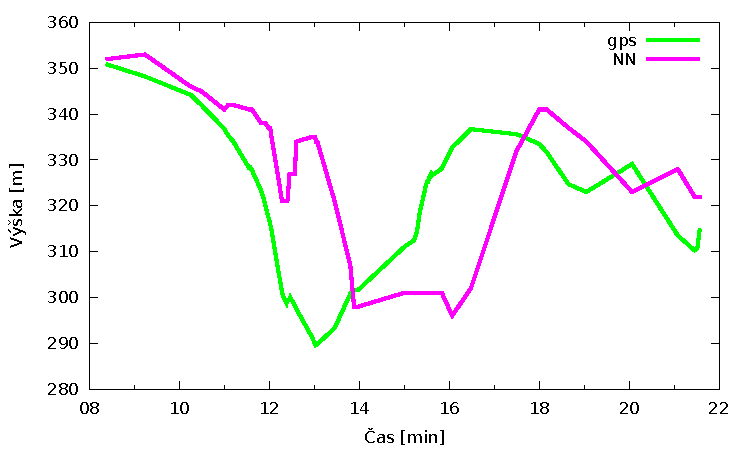
\includegraphics[page=1]{grafy/porovnani.pdf}
 	\caption{Srovnání GPS záznamu a SRTM3 dat metodou nearest-neighbour.}
 	\label{img:gpsporovnani}
 \end{figure}

 \begin{figure}[p]\centering
 	\includegraphics[page=2]{grafy/porovnani.pdf}
 	\caption{Srovnání GPS a interpolovaných SRTM3.}
 	\label{img:gpsporovnaniok}
 	
 \end{figure}


%2.2.5
%\subsection{Závislost délky trasy na jejím převýšení <<VYNECHAT?>>} 
%pythagorova věta

%2.2.6
\subsection{Rozpoznávání pauzy při záznamu trasy}
Dalším problémem při analýze tras byly pauzy. Samotná pauza se v~datech nijak výrazněji neukazuje, zkrátka se jedná o~úsek, kde se GPS záznam soustřeďuje v~mezích nepřesnosti okolo jednoho místa a většinou záznamový software nepřidává další body. Po tomto pozorování si můžeme povšimnout, že rychlost na těchto \uv{stojících} úsecích se pohybuje okolo 1 km/h. 

Řešením tedy je označení všech úseků s~rychlostí menší než 2km/h jako \uv{pauzy}, které zároveň slouží jako hranice mezi případnými minutovými intervaly, či mezi seskupenými kopci. V~analyzátoru jsou pro lepší orientaci tyto řádky označeny zvýrazněním.

%2.2.7
\subsection{Seskupování kopců}
Nyní se dostáváme k~hlavnímu účelu tohoto analyzátoru. Díky seskupení stoupajících či klesajících intervalů dostaneme souvislé úseky do kopce, resp. z~kopce. Abychom odfiltrovali malé výchylky způsobené výškovým modelem, je lepší vzít pouze rozdíl výšek dvou následujících intervalů. Následně už stačí jen spočítat procentuální převýšení kopcového úseku a vyfiltrovat ty úseky, které mají nějakou vypovídající hodnotu -- například ty, které jsou delší než 1~km.

Výsledky lze vidět v~tabulce \ref{table:vystupAnalyzatoru}, data už mají nějakou vypovídající hodnotu, ovšem jak je vidět, rychlost není závislá pouze na překonaném převýšení, ale též hraje roli například povrch, prudkost zatáček či průběh profilu.

\begin{table}[h!]
\begin{tabular}{l|l|l|l} %poslední {} v tomto řádku formátuje tabulku
\textbf{klasifikace}	&	\textbf{převýšení [m]}	&	\textbf{délka}	&	\textbf{prům. rychlost}	\\
\hline
9 \%	&	$\nearrow103$	&	1,1 km	&	6 km/h	\\
9 \%	&	$\nearrow95$	&	1,1 km	&	8 km/h	\\
7 \%	&	$\nearrow143$	&	1,9 km	&	9 km/h	\\
4 \%	&	$\nearrow40$	&	1,1 km	&	9 km/h	\\
$-2$ \%	&	$\searrow25$	&	1,3 km	&	19 km/h	\\
$-2$ \%	&	$\searrow18$	&	1,0 km	&	20 km/h	\\
$-3$ \%	&	$\searrow33$	&	1,1 km	&	20 km/h	\\
$-3$ \%	&	$\searrow35$	&	1,1 km	&	21 km/h	\\
$-6$ \%	&	$\searrow152$	&	2,7 km	&	36 km/h	\\
$-6$ \%	&	$\searrow298$	&	5,0 km	&	25 km/h	\\
$-7$ \%	&	$\searrow91$	&	1,3 km	&	17 km/h	 \\
\end{tabular}
\caption{Výstup analyzátoru pro trasu 2013-03-30.gpx (58 km, 1700 m stoupání).}
\label{table:vystupAnalyzatoru}
\end{table}


%2.2.8
\subsection{Komentář k~analyzátoru}

Na obrázku \ref{img:analyzatorScreen} vidíme reálný výstup analyzátoru části trasy 2013-03-30.gpx v~soutěsce v~obci Hřensko. Je zde vidět několik zajímavých prvků. (Vrstevnice jsou též generované ze SRTM dat.)
\begin{itemize}
%4 nejbližší pixely
\item{Zkreslení SRTM dat - datové pixely jsou reprezentovány pravidelně rozestoupenými značkami (3 úhlové vteřiny), v~místě, kde mezi nimi prochází trasa je soutěska nejužší, takže se přesně schová mezi dva nejblížší pixely. Výsledkem potom je, že interpolovaná oblast se jeví jako výše položená, v~tomto případě poslední tři kopce na výškovém grafu vpravo dole. }

\item{Zkreslení GPS signálu - výškový GPS signál je v~grafu zakreslen modrou barvou. V~tomto případě daleko věrněji kopíruje terén. Druhá polovina by měla být víceméně rovinou bez větších skoků, ty se ale v~záznamu vyskytují v~podobě artefaktů -- zkreslení dle \ref{zaznamTrasy}.}

\item{Seskupování intervalů - v~levé tabulce vidíme přesně vynesené body záznamu GPS, v~pravé části jsou seskupené do minutových intervalů.}

\end{itemize}


\begin{figure}[htp]
\centering
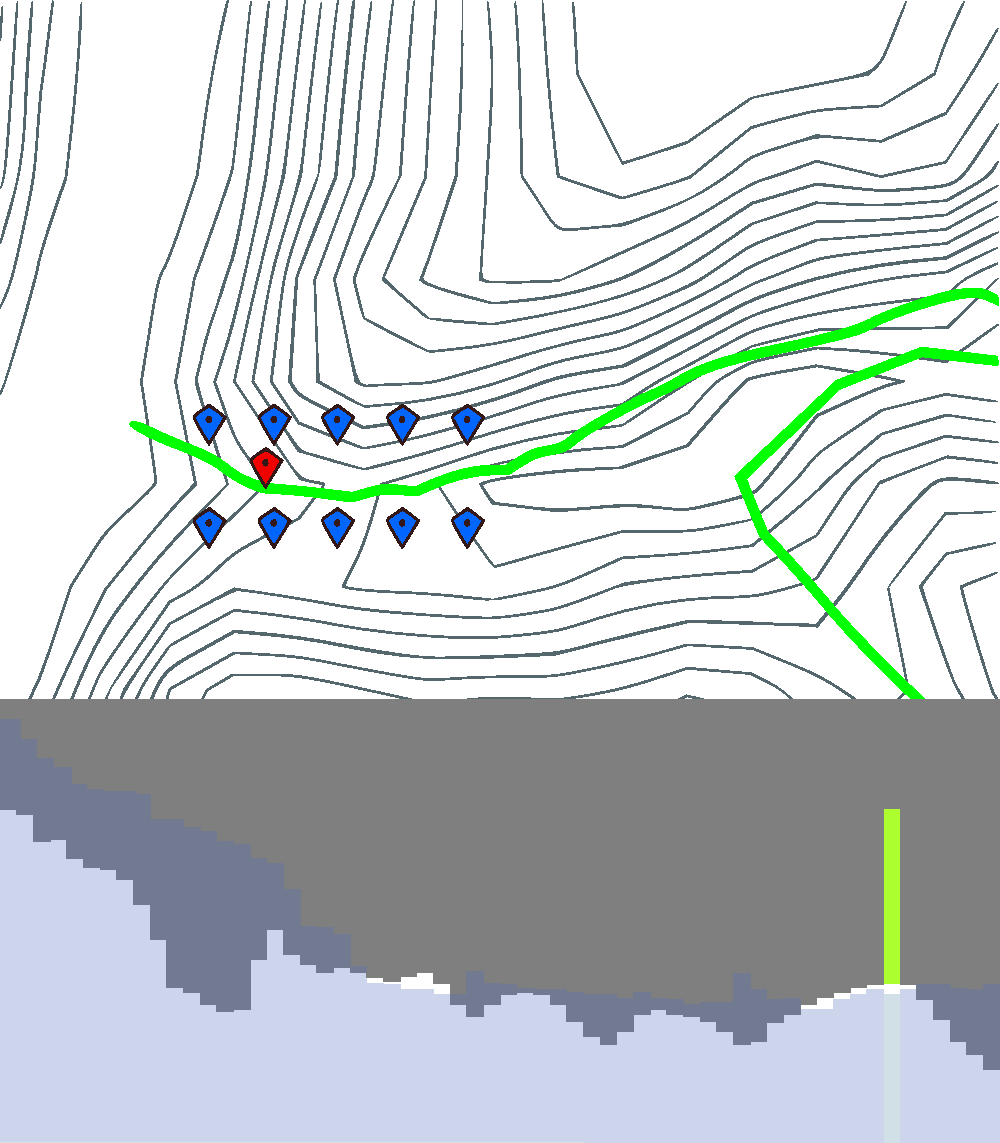
\includegraphics[width=\columnwidth,trim=0 0 0 5cm,clip]{obrazky/analyzer.pdf}
\includegraphics[width=\columnwidth,page=2,trim=1.2cm 11.5cm 6cm 10.3cm,clip]{obrazky/analyzer-tabulka.pdf}
\caption{Screenshot analyzátoru demonstrující zkreslení GPS a zemského modelu.}
\label{img:analyzatorScreen}
\end{figure}


\subsection{Komentář k~výškovému modelu}

Na sérii obrázků \ref{img:hrensko} vidíme 3D vizualizaci stejné trasy v~digitálních modelech Země. Všechny grafy jsou vynesené do kartézské soustavy, ačkoliv souřadnice jsou z~polárního systému. Díky tomu můžeme pozorovat asi dvojnásobné zvětšení v~ose Y, ovšem prostorové zkreslení díky malým délkám není vůbec viditelné. 

Pohled je položen vůči mapě od \uv{severozápadu}, ovšem kvůli přehlednosti vizualizovaného problému musela být invertována osa Y a doopravdy jsou tedy sever a jih prohozeny. Kvůli zvyklosti zobrazování map je tento fakt matoucí a tedy je lépe si ho neuvědomovat. Díky tomu, že trasa vede východo-západně, není inverze osy Y problematická.

Trasa je vynesena ve dvou výškách -- modrá nese výšková data přímo z~analyzéru, tedy SRTM3 od CGIAR, tyrkysová jsou data z~GPS zařízení. Jak vyplývá i z~analyzéru, je zde podezření, že výšková data z~GPS jsou kvůli skalnatému okolí v~celém průběhu posunuta až o~20 m výše.

Na všech grafech je označen černým křížkem zvýrazněný bod z~analyzátoru.

První model jsou data ASTER GDEM, díky rozlišení 1 úhlové vteřiny jsou data výrazně podrobnější a nám poslouží jako referenční model. Kvůli novému měření a vynechanému průměrování je také více plastická do hloubky i do výšky. V~horním zákrutu je vidět větší vzdélnost od obou tras, přibližně 30 m.

Druhý a třetí model ukazují data SRTM3, kde vidíme, že průměrování výšek ubralo na plastičnosti. Druhý model ještě zvýrazňuje model soutěsky ve směru osy Y, tedy jsou daleko snáze vidět datové body SRTM.

Pravděpodobně kvůli jiným interpolačním technikám programu Gnuplot a SRTM parseru v~analyzéru se trasa místy vyskytuje pod 3D povrchem.



\begin{figure}[]
\centering
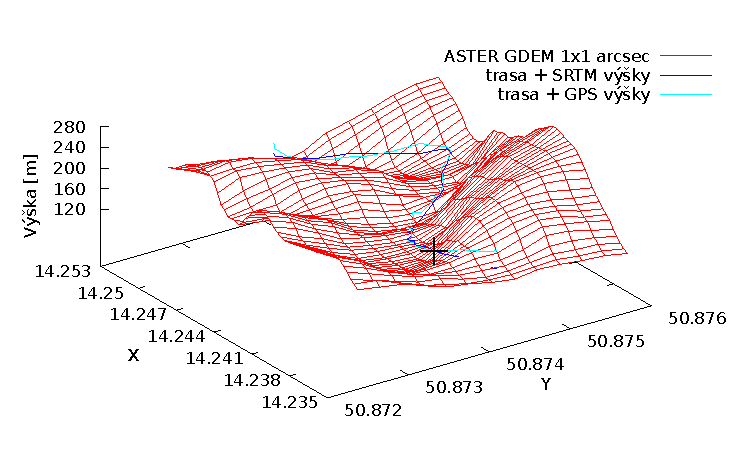
\includegraphics[width=130mm,trim=0 5mm 0 10mm]{grafy/3D-aster1.pdf}
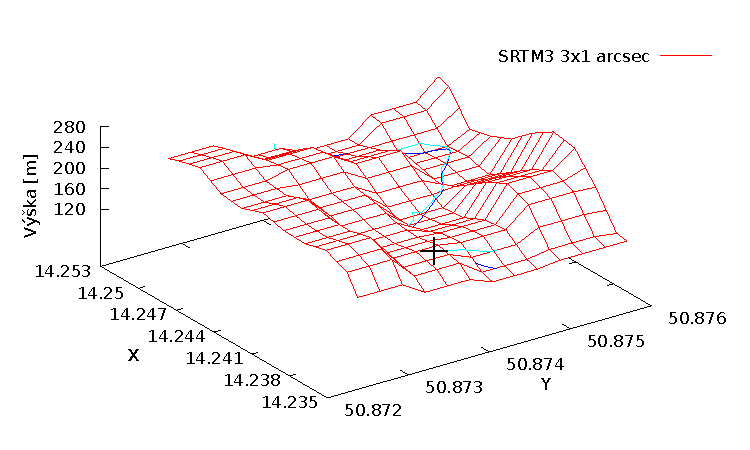
\includegraphics[width=130mm,trim=0 5mm 0 5mm]{grafy/3D-srtm3x1.pdf}
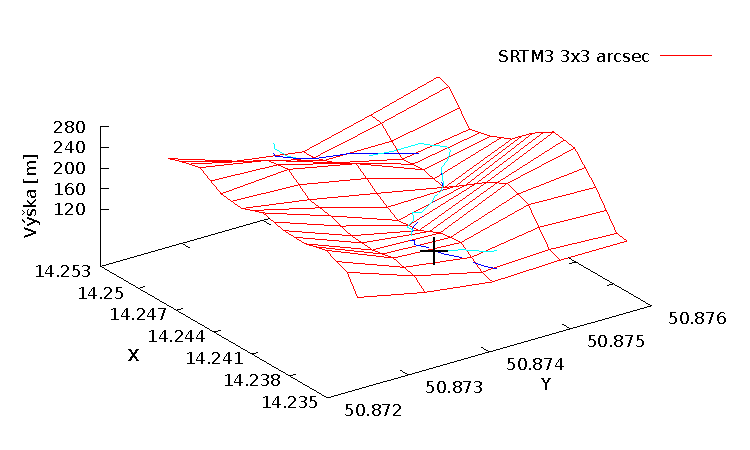
\includegraphics[width=130mm,trim=0 5mm 0 5mm]{grafy/3D-srtm3.pdf}
\caption{Ilustrace zkreslení způsobeného rozlišením SRTM dat a jejich interpolací. }
\label{img:hrensko}
\end{figure}








%2.3---------------------------------------------------------
%---------------------------------------------------------
\section{Model cyklisty}
%---------------------------------------------------------
Zdá se tedy, že určit rychlosti dle klasifikace kopců již bude snadné. Též každý cyklista může využít analyzátor a určit si své vlastní rychlosti. Celkově zůstanou hodnoty spíše orientační, ale již je to odhad, se kterým lze dále pracovat.

Není tedy zatím v~našich silách automaticky spočítat patřičné klasifikace kopců přímo z~nahraných dat. Automaticky funguje vymazání pauz, seskupení kopců a napočítání charakteristik. Kvůli nepřesnostem je ale pak na uživateli, aby vyhodnotil relevantní úseky a nepočítal ty, kde chyba měření způsobuje nesmyslené výsledky.
























%3.---------------------------------------------------------
%---------------------------------------------------------
\chapter{Implementace}
%---------------------------------------------------------
%---------------------------------------------------------
Ačkoliv jsme si ověřili, že existuje mnoho systému, do kterých lze výškovou optimalizaci přidělat, je zde také varianta napsání systému zcela vlastního.

Vlastní řešení by spočívalo jednak v~přípravě dat. OpenStreetMap data jsou dostupná ve formátu XML, odkud je lze snadno použít. Graf mapové sítě je velmi řídký a pro routování si není nutné držet geometrii cesty, můžeme tedy provést kompresi hran až po křižovatky a geometrii nechat pouze jako doplňkový údaj ke každé hraně. Dále by bylo potřeba zvolit vlastní databázové řešení a implementovat samotný vyhledávací algoritmus.

Vzhledem k~tomu, že tato práce se zabývá především minimalizací převýšení, byl s~ohledem na rešerši v~kapitole \ref{porovnaniSystemu} zvolen systém Routino.


%3.1---------------------------------------------------------
%---------------------------------------------------------
\section{Infrastruktura routeru Routino}
%---------------------------------------------------------
%---------------------------------------------------------

Celý softwarový balík se dělí na několik programů.
\begin{itemize}
	\item{\verb|planetsplitter| -- parsuje vstupní OSM datové soubory v~různých formátech a ukládá je do vnitřních datových struktur a následně do externích souborů. Zvládá též integraci tzv. souborů změn do existujícíh struktur. }
	\item{\verb|router| -- na základě vstupních argumentů a souborů s~datovými strukturami hledá nejkratší nebo nejrychlejší trasu a vypisuje výstup v~několika formátech.}
\end{itemize}	

Toto dva nástroje existují ještě ve formě \verb|slim|, která místo načítání do operační paměti pomocí memory-mapped file využívá pouhé posouvání ukazatele v~souborech (seekování). Tedy je vhodná i pro systémy s~velmi omezenými prostředky. Následující programy jsou pouze doplňkové.

\begin{itemize}
	\item{\verb|filedumper| -- dokáže z~datových struktur vygenerovat opět OSM XML, také vypisuje statistické informace o~souborech. Ve webové verzi je k~němu rozhraní na stránce \verb|visualiser.html|}
	\item{\verb|tagmodifier| -- upravuje zadaný OSM XML soubor, tak že z~něj dle daných pravidel tagging.xml odebere nepotřebné prvky.}
\end{itemize}


%3.1.1
\subsection{OpenStreetMap data}
Soubor OSM XML je stejně jako OSM data tvořen třemi datovými primitivy, každý obsahuje též referenční číslo (ID).

 Uzly (nodes) jako jediné nesou informaci o~zeměpisné poloze, volitelně mají též navázany atributy (tags), např. semafor, přechod, závora. 
 
 Cesty (ways) seskupují více uzlů v~daném pořadí, atributy popisují např. typ cesty, omezení maximální rychlost, povolené dopravní prostředky či prosté jméno ulice. Pokud je první uzel stejný jako poslední, je cesta uzavřená a některé vlastnosti z~ní tak mohou vytvořit plošný objekt.
 
 Relace (relations) seskupují více uzlů a cest s~danými rolemi. Pro routování má smysl především relace zákazů odbočení, které udavají mezi kterými cestami je zákaz.
 

%TODO jak zformátovat popisek k textu?
{Příklad OSM XML souboru:}
\begin{verbatim}

<node id="2270977371" version="1" changeset="15765764" 
 lat="50.0" lon="14.3" user="zby-cz" uid="162287" 
 visible="true" timestamp="2013-04-17T18:41:18Z"/>

<way id="217792329" visible="true" timestamp="..." 
 version="1" changeset="15765764" user="zby-cz" uid="162287">
    <nd ref="2270977371"/>
    ...
    <tag k="highway" v="motorway"/>
</way>
\end{verbatim}


Jiné formáty jsou OSM PBF a O5M. První využivá tzv. Google Protocol Buffer Binary Format, který v~zásadě zapisuje XML binárně do bloků, které mohou být i seskupeny dle geografických souřadnic. Též provádí gzip kompresi. Druhý formát je novější a navíc funguje streamově stejně jako původní XML, volba komprese je pak na uživateli.



%---------------------------------------------------------
\subsection{Datové struktury a načítání}
Datové struktury Routina v~podstatě kopírují primitivní typy OSM. Navíc kvůli routování je přidána struktura Segments -- to jsou úseky mezi dvěma uzly, které rovnou nesou i délkové ohodnocení. 

Nejdříve jsou primitiva uložena s~původními referenčními ID. Uložení formátu OSM XML zajišťuje, že jsou ID seřazena v~neklesající posloupnost, ale tento invariant je raději zajištěn seřazením. 

Aby fungoval i zmíněný \verb|slim| režim, odkazování na reference je zajištěno metodou půlení intervalů. Toto by samozřejmě při vyhledávání bylo velmi pomalé, a tak funkce \verb|MeasureSegments| jednak přidá segmentům délkové ohodnocení (vyhledá oba uzly, zjistí jejich souřadnice a haversinovou formulí změří vzdálenost) a také přečísluje ID na pořadová čísla.

Přečíslování umožňuje random-access pomocí pointerové aritmetiky a následně je tedy využito pro vytvoření spojových seznamů následníků pro každý uzel. Aby se minimalizovaly čtecí přístupy, je seznam distribuovaný přímo do odkazovaných prvků. Tedy uzel má uloženo pořadové číslo prvního segmentu z~následníků a segment má číslo druhého, atd.


%3.1.3---------------------------------------------------------
\subsection{Super segments}
\label{super-segments}
Kvůli zrychlení vyhledávání se používá ještě jedna zajímavá technika a tou je slučování hran v~\uv{super hrany}. V~několika iteracích se vždy sousední segmenty sloučí, pokud by mezi nimi neležel tzv. \uv{super uzel}, tedy takový uzel, jež mění typ cesty, obsahuje bariéru či další odbočky, viz obrázek \ref{img:superhrany}, převzato z~\cite{routino-doc}.

Důležité je, že super segmenty se vytvoří pro každou hranu, tedy některé vlastně jen zduplikují, pro routování se následně využívá pouze tento super graf.

Pro nás je toto místo důležité, protože je třeba zachovat parametry převýšení z~původních segmentů do těchto nově vzniklých.

\begin{figure}[!ht]
\centering
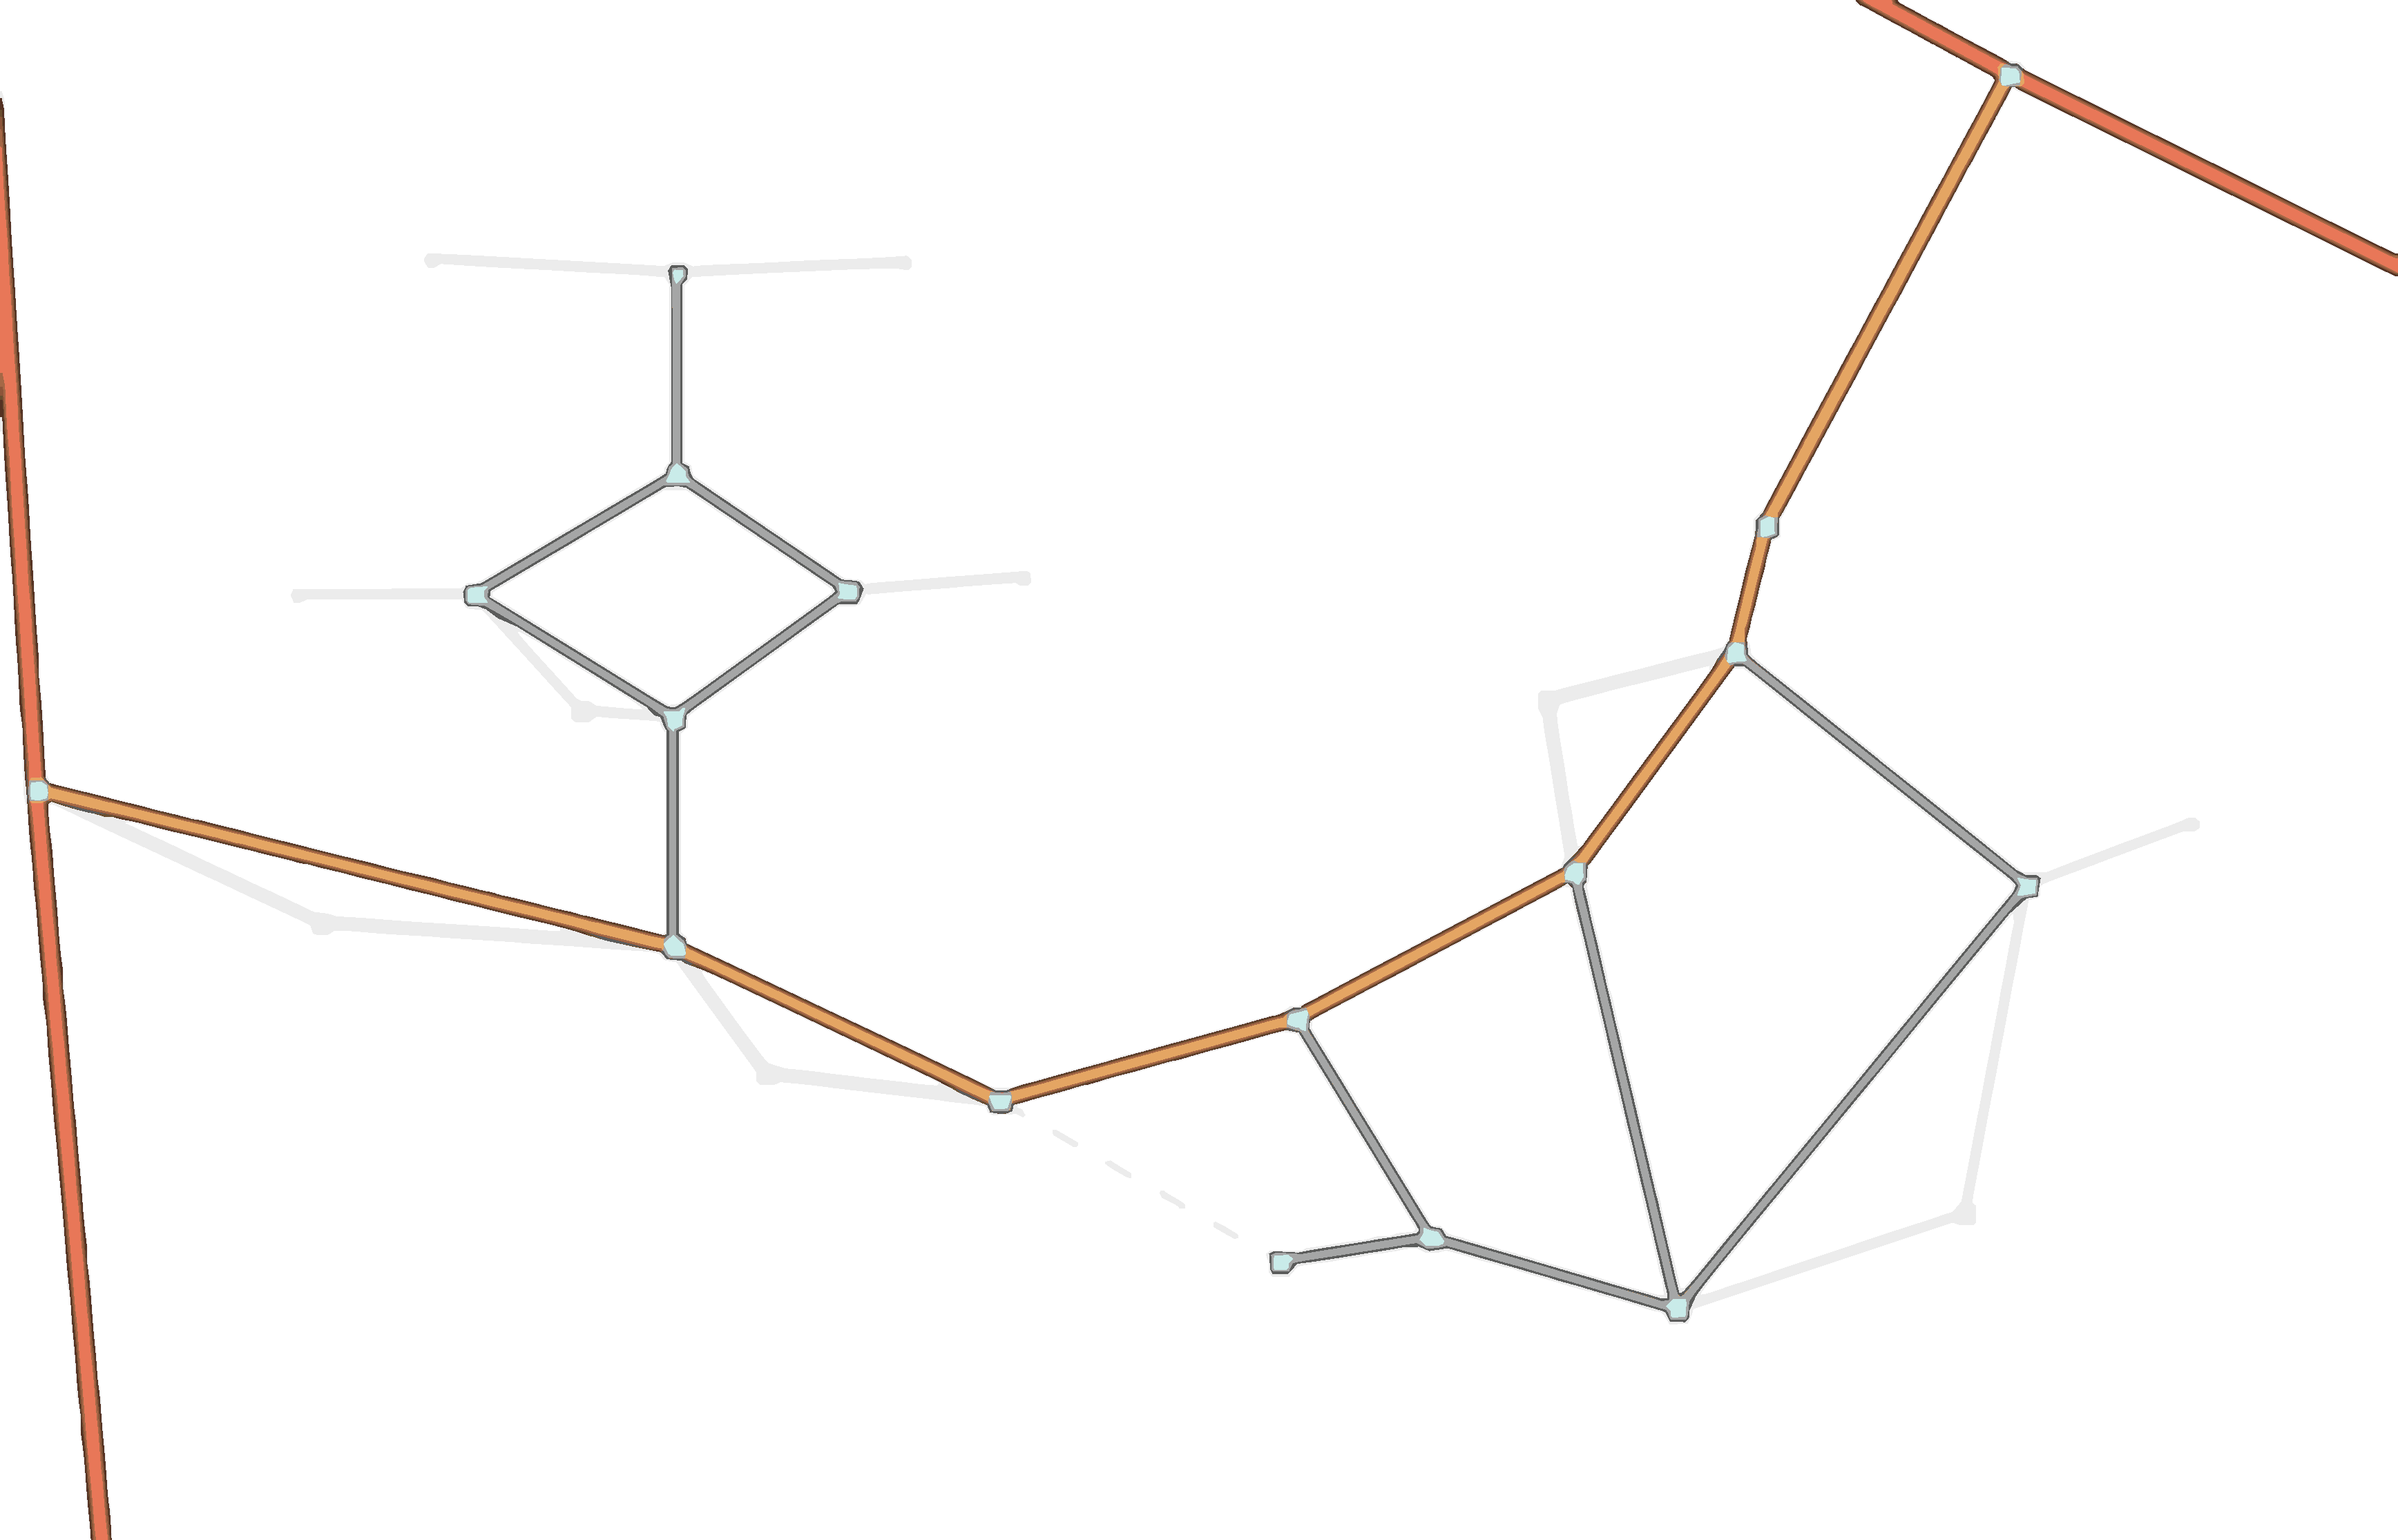
\includegraphics[width=\columnwidth]{obrazky/supernodes.pdf}
\caption{Ilustrace komprese hran v~super-hrany }
\label{img:superhrany}
\end{figure}



%3.1.4---------------------------------------------------------
\subsection{Vyhledávací algoritmus}
\label{vyhledavaci-algoritmus}
Program \verb|router| pracuje též v~příkazové řádce. Na vstupu dostává souřadnice průjezdních bodů. V~první části algoritmu se prochází celá databáze a hledá se nejbližší uzel pro každý průjezdní bod. Aby se celá operace urychlila, jsou uzly uložené ve skupině (bins) s~blízkou zeměpisnou souřadnicí a pokud je souřadnice skupiny příliš daleko, ihned se přeskočí.

V~druhé části se hledá cesta od startovního uzlu do prvního super-node. Následující hledání je již po super-grafu, tedy s~využitím super-segments.
Může se stát, že místo super-node je přímo nalezen cílový uzel, potom se část routování přes super-segments nekoná.

Ačkoliv to není nikde zmíněno používá se pro hledání algoritmus A*, definovaný jako rozšíření Dijkstrova algoritmu v~článku~\cite{astar}. Nejprve se založí nová struktura typu \verb|Result|, která nese hranu s~navazujícím uzlem pro startovní bod.

Následně je vložena do prioritní fronty a seřazeny podle vlastnosti \emph{sortby}, která využívá heuristiku \emph{skóre} + \emph{odhad vzdálenosti do cíle}. Samotná prioritní fronta je implementována binární haldou.

Další vlastnost je \emph{skóre}. To je nejzásadnější parametr pro vyhledanou trasu, ten se snaží algoritmus minimalizovat. Podle toho jestli hledáme nejkratší či nejrychlejší trasu, obsahuje vzdálenost, resp. čas na trase. Kromě toho je ještě skóre nepřímo úměrné \emph{preferenci} vázané na typ cesty.

Každá iterace vždy odebere nejníže ohodnocený výsledek a z~jeho uzlu iteruje přes všechny sousední hrany. Pokud byl již sousední uzel navštíven, je upraven pouze tehdy, pokud má nižší skóre.

Pakliže je nalezena trasa do cílového uzlu (výsledek měl nejnižší \emph{sortby}), tak už má smysl rozvíjet pouze ty výsledky, jejihž \emph{skóre} nepřekoná \emph{skóre} dosažené trasy. Tím je zajištěna minimalita nalezené trasy.

%3.1.5---------------------------------------------------------
\subsection{Nasazení Routino jako webové služby}
Vzhledem k~tomu, že celá práce směřuje k~připravě webové služby, je dobré prozkoumat, jaké možnosti nabízí systém Routino. 

Již v~distribučním archivu se nalézá složka \verb|web|. Po kompilaci se do podsložky \verb|bin| zkopírují binární programy, v~podsložce \verb|data| jsou připravena pravidla pro ukládání tagů \verb|tagging.xml| a skript pro stažení vektorových OSM dat. V~této složce se tedy spustí výše popsaný program \verb|planetsplitter|, který zpracuje data pro routování a uloží do souborů \verb|nodes, segments, way| a \verb|relations.mem|. 

V~podsložce \verb|www| je potom funkční webová aplikace, která obsahuje spouštěcí formulář pro cgi službu, ve které je třeba nakonfigurovat dostupnost programu \verb|router|. Data se následně ukládají do podsložky \verb|results| odkud si je webová aplikace načte ve formátu GPX. Aplikace je postavena nad javascriptovou mapovou knihovnou OpenLayers \cite{openlayers}.



%3.2 ---------------------------------------------------------
%---------------------------------------------------------
\section{Úprava algoritmů a datových struktur}
\label{uprava-algoritmu}
%---------------------------------------------------------
%---------------------------------------------------------
Nyní se dostáváme k~samotné části implementace. Do fungujícího programu a algoritmů bude třeba přidat informaci o~nadmořské výšce a následně ji zakomponovat do skóre hran.

Nejprve je potřeba stanovit jaká data vlastně u~jakých struktur potřebujeme a následně můžeme navrhnout datový model. Smysl má uvažovat pouze o~uzlech a segmentech, neboť ty vystupují jako graf při samotném routování.

Když si projdeme fuknce vyhledávající na grafu a následně super-grafu (podrobně kapitola \ref{vyhledavaci-algoritmus}) jsou tu při každé iteraci  v~režimu \uv{nejrychlejší trasa} skóre hran hodnoceny funkcí \verb|Duration(Way, Segment, Profile)|, při volání je k~dispozici také výchozí uzel \verb|node1|, druhý lze dohledat přes segment.

První myšlenka by mohla při routování se dotazovat na nadmořskou výšku každého uzlu a počítat rozdíl pro každý segment. Tento přístup má dvě nevýhody. Jednak by pro každý uzel musel být otevřen a přečten soubor s~výškovými daty -- což by nejspíše 2-$5\times$ zpomalilo hledání. Druhá nevýhoda ale činí toto řešení nepoužitelným -- při spojování hran do super-hran (podkapitola \ref{super-segments}) totiž ztrácíme informaci o~vnitřních uzlech.

Řešením tedy rozhodně je číst výšková data už při načítání, tedy upravit \verb|planetsplitter| a s~ním i datové struktury. Tím odstraníme první nevýhodu, ovšem druhou musíme vyřešit jinak. 

Nabízí se ukládat k~segmentům sumu nastoupané a naklesané výšky, ovšem abychom zde mohli klasifikovat kopce, je ještě nutné uložit na jaké vzdálenosti se stoupalo, resp. klesalo. 

Pokud je úbytek rychlosti v~přímé úměrnosti s~klasifikací kopce, budou výsledky úplně přesné. Pokud ovšem bude charakterstika jiná, bude zde jisté zkreslení díky možnému seskupení více kopců. Je dobré mít na paměti, že analyzér se dopouští přibližně stejné chyby, neboť kopce také seskupuje a následně počítá jejich klasfikaci.

Výsledná klasifikace kopců byla zvolena dle výstupu z analyzéru dle tabulky \ref{table:vystupAnalyzatoru}, nastavit tyto hodnoty je možné přímo ve funkci \verb|Duration|, konkrétní hodnoty jsou v tabulce \ref{table:hodnoty}


\begin{table}[h!]
\begin{tabular}{l|l} %poslední {} v tomto řádku formátuje tabulku
\textbf{klasifikace}	& \textbf{výsledná rychlost}	\\
\hline
0-2 \%	&	20 km/h	\\
2-4 \%	&	15 km/h	\\
4-7 \%	&	10 km/h	\\
7-9 \%	&	8 km/h	\\
9-15 \%	&	6 km/h	\\
15 a více \%	&	3 km/h	\\
\end{tabular}
\caption{Nastavení ohodnocení stoupajících hran v Routinu.}
\label{table:hodnoty}
\end{table}





% 3.3 ---------------------------------------------------------
%---------------------------------------------------------
\section{Heuristika pro hledání trasy}
%---------------------------------------------------------
%---------------------------------------------------------
Jak jsme již zmínili v~podkapitole \ref{vyhledavaci-algoritmus}, je heuristika u~běžného vyhledávání zajištěna odhadem vzdálenosti, resp. času na přímočaré spojnici z~dotyčného bodu do cíle.

Pojďme se zamyslet, jak by tento způsob šel přenést na odhad převýšení do cíle. 

Jistě by bylo možné spočítat též převýšení na přímočaré spojnici, má to ale několik nedostatků. Jednak technicky tato data nelze získat z~žádné předzpracované databáze a bylo by nutné je všechny dotázat, což je zásadní zpomalení, když vezmeme v~potaz, že každý uzel je získán jedním čtením souboru a odhad výšky by obsahoval až tisíce čtení.

Druhý problém je zásadnější, jedná s~o~samotnou kvalitu takového odhadu. Cesty v~reálném světě jsou zpravidla vedeny po vrstevnicích spíše než přímočare, tak aby stavitelé právě nemuseli překonávat přílišné převýšení. Náš odhad by tak neměl nic společného s~realitou a nemohl by způsobit prokazatelné zrychlení algoritmu. Tuto cestu tedy zavrhneme.

Další myšlenka je jednodušší. Pokud bychom vzali nadmořskou výšku aktuálního bodu a nadmořskou výšku cíle, bylo by možné odhadnutý čas založit na rychlostním odhadu stoupání či klesání. 

Problémy jsou opět nasnadě. Ačkoliv zde platí, že výškový rozdíl bude třeba překonat, výsledný čas bude velmi záležet na sklonu. K~tomu připočtěme neznámý počet kopců do cíle a zjistíme, že i takový odhad je velice špatný. Praktického využití bychom dosáhli možná v~krajině, která obsahuje náhorní plošinu, ale menší množství kopců. Stále ovšem platí, že heurstika založená pouze na vzdálenosti má výsledky dostačující.


% 3.4 ---------------------------------------------------------
%---------------------------------------------------------
\section{SRTM reader}
%---------------------------------------------------------
%---------------------------------------------------------
Doposud jsme mluvili o~načítání výškových dat, ovšem řešení tohoto problému není zcela triviální. Routery tuto funkci zpravidla neobsahují a ani se nepovedlo nalézt volně dostupnou implementaci v~jazyce C, kterou by bylo možné využít. Inspirací byl PHP reader (viz \cite{osola}) a komponenta GrassGISu v.drape (viz \cite{grassgis}). Celou implementaci jsme zveřejnili na serveru GitHub: \\  \href{https://github.com/zbycz/srtm-hgt-reader}{http://github.com/zbycz/srtm-hgt-reader}



%---------------------------------------------------------
\subsection{Formát dat a konverze}

Jak jsme zmínili v~podkapitole \ref{dem}, jsou výšková data dostupná buď ve formátu GeoTIFF nebo HGT. Soubory jsou uskupeny do dlaždic, které jsou zpravidla pojmenovány decimální částí souřadnic a obsahují tak vždy celý úhlový stupeň zeměpisné šířky i délky. Podle rozlišení 1 nebo 3 úhlové vteřiny pak obsahuje 3601 nebo 1201 hodnot do řádků i sloupců.

Formát GeoTIFF se využívá na rozličné uchování rastrových dat se zakódovanými souřadnicemi a typem mapové projekce. Díky robustnímu řešení je načítání poměrně obtížné a zabývá se jím obsáhlá knihovna libtiff \cite{libtiff}. Samotná výšková data jsou z~povahy SRTM uloženy jako dvoubajtové signed integery, kde hodnota $-32768$ znamená nedefinovaná data.

Formát HGT je zásadně jednodušší. Nemá žádnou hlavičku ani kódování souřadnic a projekcí. Obsahuje pouze datovou oblast, kde se nachází stanovený počet dvoubajtových integerů a tak jediným problémem může být správně dekódovat endianitu. Souřadnice se pak odvíjejí pouze od pojmenování souborů. Přesný popis formátu v~\cite{srtm-manual}. 

Podívejme se ještě na interpolaci dat a počítání převýšení dle požadavku routeru v~podkapitole \ref{uprava-algoritmu}.


%---------------------------------------------------------
\subsection{Bilineární interpolace dat}
Jak je patrné z~obrázků \ref{img:gpsporovnani} a \ref{img:gpsporovnaniok}, bez interpolace dat se neobejdeme. 

Bilineární interpolace vezme 4 nejbližší body a sečte hodnotu všech těchto bodů vždy přenásobené koeficienty, které určují poměr vzdáleností. Výsledek interpolace je vidět na obrázku \ref{img:interpolace}.


%TODO
Kvůli rychlosti se obvykle používá právě bilineární interpolace, ačkoliv existují i interpolace vyšších řádů. Zde stačí získat pouze malé množství bodů a provést výpočetně snazší operace. Zde se také vysvětluje, proč všechny nabízené formáty výškových dat obsahují ještě horní a pravý sloupec zduplikovaný z~vedlejších dlaždic. Důvodem je právě možnost snadné bilineární interpolace bez nutnosti mít současně otevřené v~paměti dvě dlaždice výškových dat.

V~naší implementaci jsme použili následující vzorec pro interpolaci dat, kde $d_x$ a $d_y$ jsou poměry polohy určovaného bodu v~x-ové a y-ové souřadnici:

$h_{0,1} * d_y * (1 - d_x) + h_{1,1} * d_y * (d_x) + $

$h_{1,0} * (1 - d_y) * d_x + h_{0,0} * (1 - d_y) * (1 - d_x) $



\begin{figure}[]
\centering
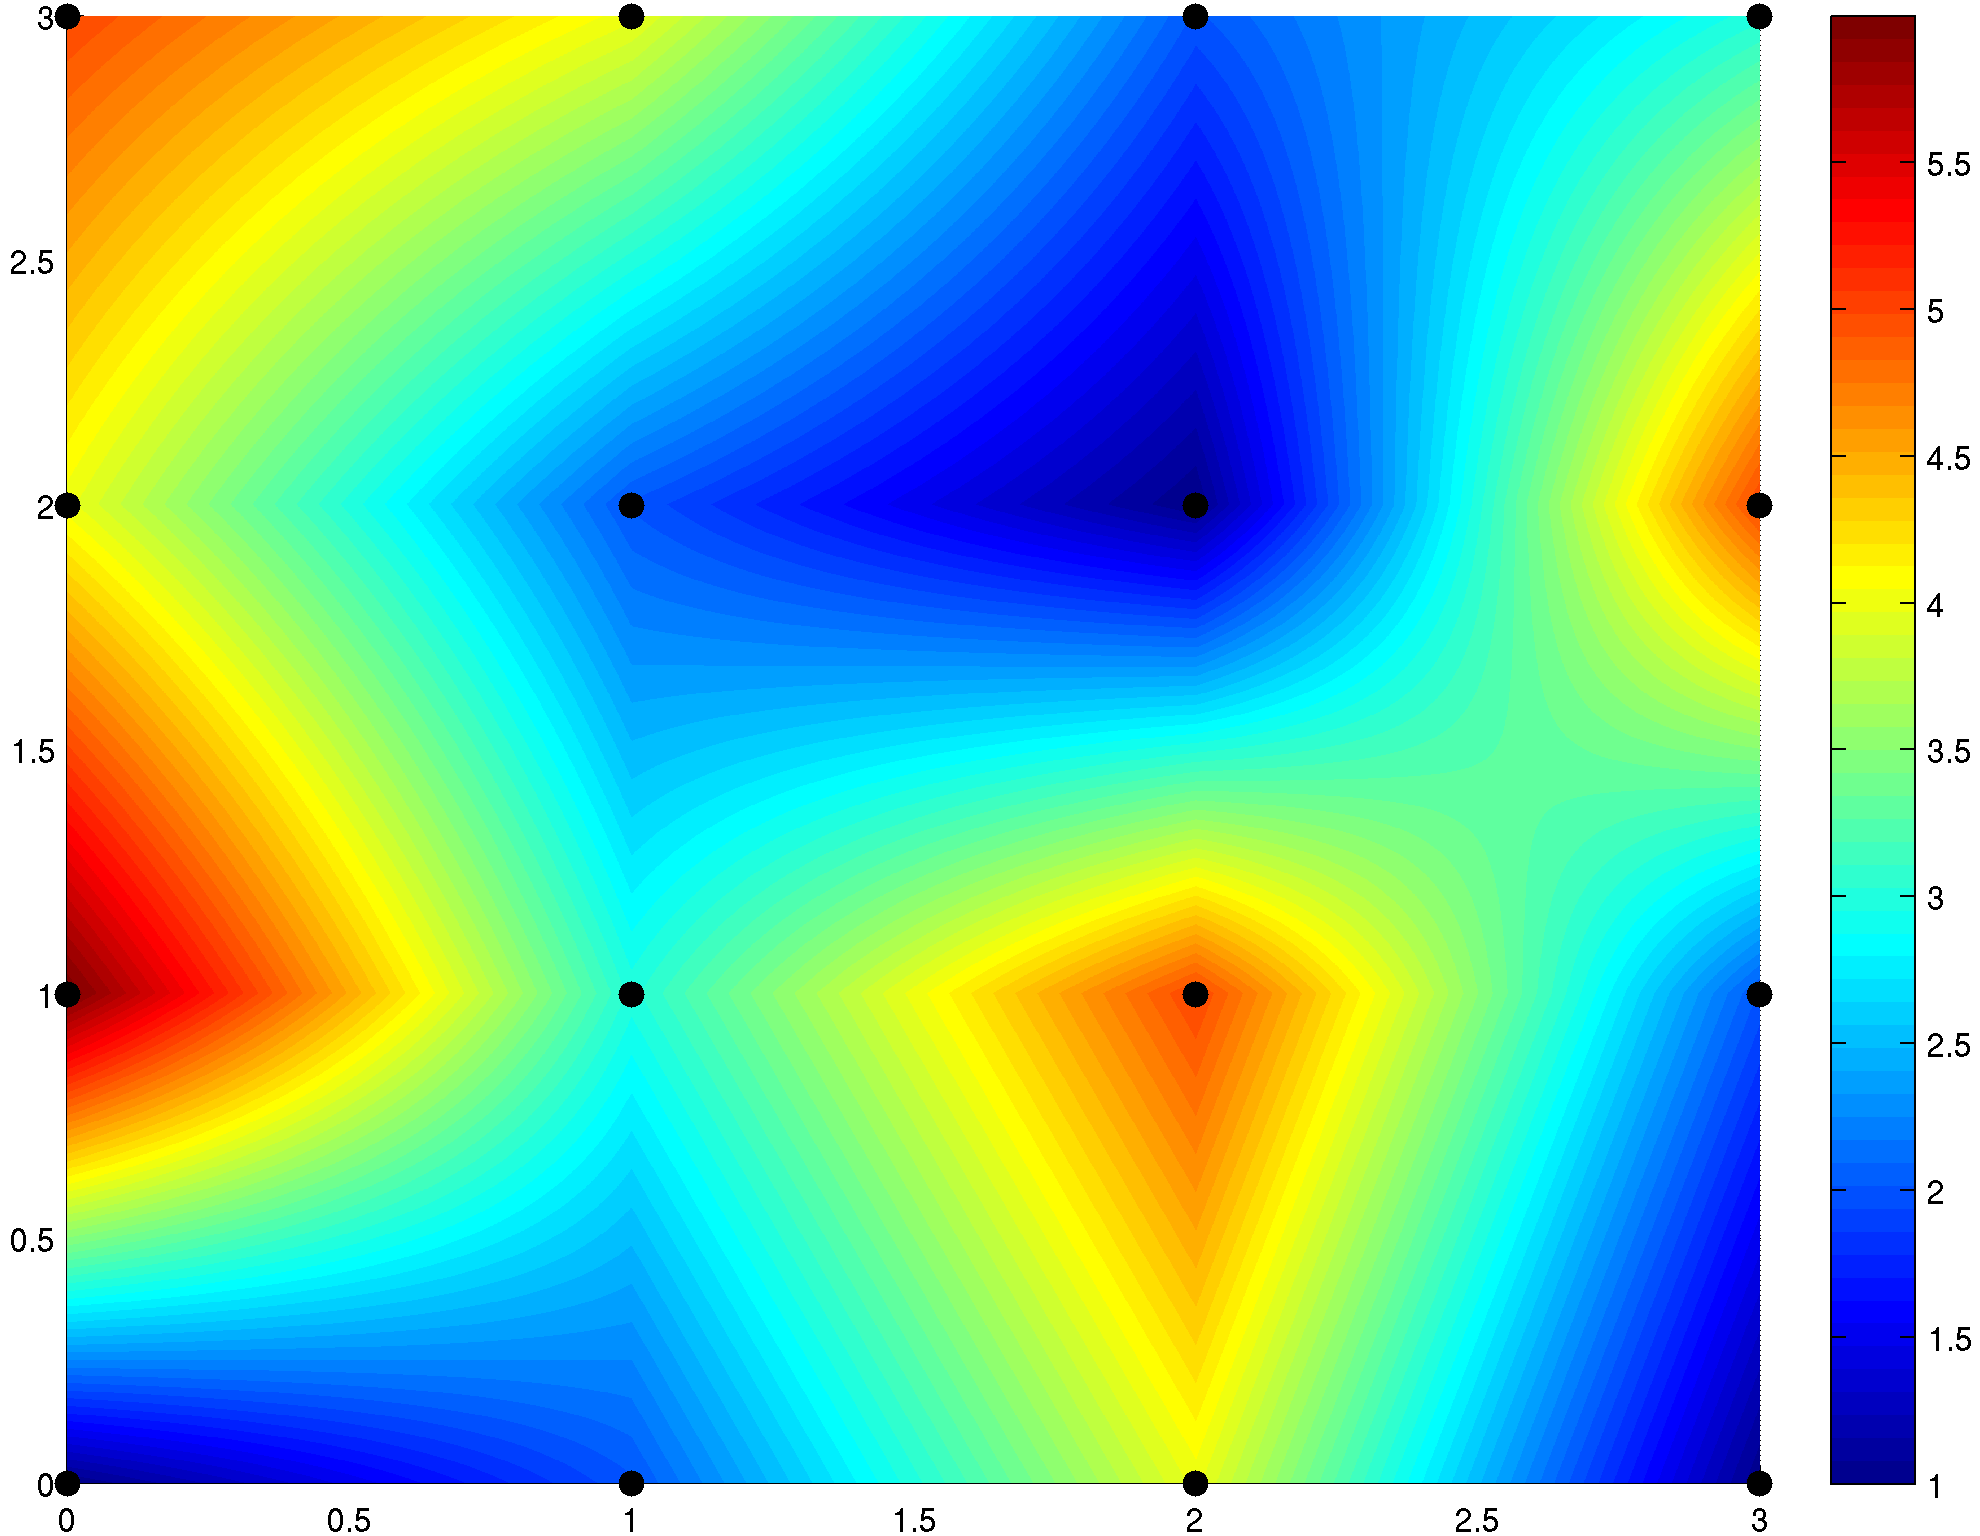
\includegraphics[width=\textwidth]{obrazky/bilinearni-interpolace.png}
\caption{Vizualizace dat s~bilineární interpolací v~programu Matlab. }
\label{img:interpolace}
\end{figure}



%---------------------------------------------------------
\subsection{Výstup SRTM readeru}
Kromě zjišťování interpolované polohy jednoho bodu umí reader také vypočítat nasčítané převýšení na zadané přímočaré spojnici. Kvůli paměťovým nárokům se lze přepnout do režimu SLIM (zadefinováním stejnojmenného makra), kdy reader nenačítá celou HGT dlaždici do paměti, ale pouze v~ní seekuje na určené místo.

Veřejné programátorské rozhraní v~jazyce C obsahuje tyto funkce:
\begin{itemize}

\item{float srtmGetElevation(float lat, float lon); \\
Základní volání pro zjištění jednoho bodu udaného v~decimálních stupních.}

\item{void srtmClose(); \\
Ukončení práce s~readerem a uvolnění alokovaných zdrojů.}

\item{TSrtmAscentDescent srtmGetAscentDescent(latlon1,2 ..., dist); \\ 
 Funkce přímo pro použítí v~routeru. Dotazuje všechny pixely ležící mezi dvěma zadanými body a stoupání a klesání vrací ve struktuře, která obsahuje také poměr vzdálenosti (dist), na které proběhla stoupací část a klesací.
 }

\end{itemize}



%---------------------------------------------------------
%---------------------------------------------------------
\section{Využití SRTM readeru v~systému Routino}
%---------------------------------------------------------
%---------------------------------------------------------

Jak jsme zmínili v~podkapitole \ref{uprava-algoritmu}, je nutné využít funkci pro získání převýšení na každém segmentu. Ta se volá ve fázi \verb|MeasureDistance|, kdy jsou ještě segmenty v~načítací struktuře (tzv. SegmentX) a jsou tedy k~dispozici snadno čitelné zeměpisné souřadnice. Získaná struktura se uloží ke každému segmentu a na super-segmentech je agregována.





















%---------------------------------------------------------
%---------------------------------------------------------
\chapter{Zhodnocení výsledků}
%---------------------------------------------------------
%---------------------------------------------------------

Pro porovnání výsledků jsme vybrali dvě trasy, jejihž přímá cesta vede přes kopec. Můžeme si všimnout, že námi upravený systém Routino hledal původně trasy podobně jako ostatní systémy. Upravená verze zohledňuje kopce a dosahuje podobně dobrých výsledků jako BRouter. V tabulkách se nachází přehled všech systémů, na  obrázcích jsou kvůli přehlednosti vybrány jen některé. 

Vstupní data jsme získali pomocí úpraveného analyzéru projetých tras z~kapitoly \ref{routovani}, výstup zajištěn programem Gnuplot.

\section{Trasa přes Haunspaulku}
Z tabulky \ref{table:h} vidíme, že optimalizace převýšení je na úkor délky. Na obrázku \ref{img:vyska-h} a \ref{img:mapa-h} splývají trasy ze systému Cloudmade a původního Routina, neboť tato trasa je shodná. 


\begin{table}[h!]
\begin{tabular}{l|l|l|l} %poslední {} v tomto řádku formátuje tabulku
\textbf{systém}	&	\textbf{délka [m]}	&	\textbf{stoupání [m]}	&	\textbf{klesání [m]}	\\
\hline
BBBike	&	3083 & 124	&	29	 \\
BRouter	&	3991 & 104	&	9	 \\
Cloudmade	&	2946 & 118	&	23	 \\
Mapy.cz	&	2956 & 122	&	27	 \\
OpenRouteService	&	3238 & 120	&	25	 \\
Routino původní	&	2939 & 118	&	23	 \\
Routino upravené	&	3806 & 102	&	7	 \\
YOURS	&	3383 & 127	&	32	 \\
\end{tabular}
\caption{Porovnání všech dostupných routerů.}
\label{table:h}
\end{table}

\begin{figure}[!ht]
\centering
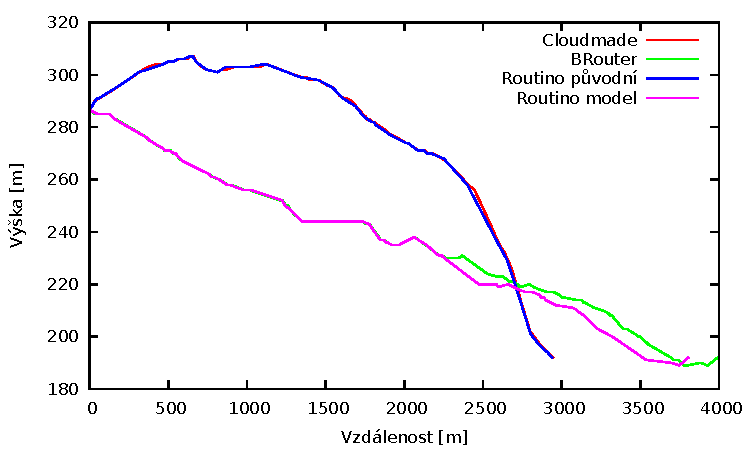
\includegraphics[width=\columnwidth]{porovnani/ele-2h-z.pdf}
\caption{Nadmořská výška vyhledaných tras dle SRTM. }
\label{img:vyska-h}
\end{figure}

\begin{figure}[!ht]
\centering
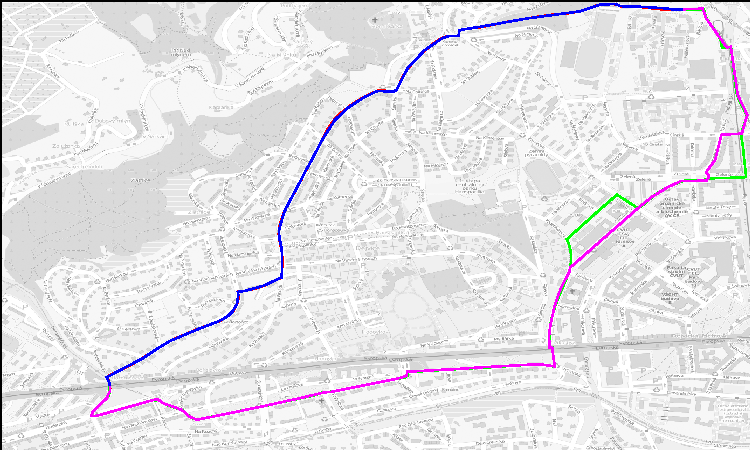
\includegraphics[width=\columnwidth]{porovnani/ll-2h-z.pdf}
\caption{Zobrazení nad OpenStreetMap podkladem. }
\label{img:mapa-h}
\end{figure}






\section{Trasa z Nuslí do Podolí}
Druhá trasa je nastavena tak, aby přímá spojnice vedla přes Vyšehrad. Zajímavé je, že Cloudmade zde nalezl kratší cestu než původní Routino, ovšem obojí vede přes kopec, jak je vidět na obrázku \ref{img:vyska-n}. 

Obě výškově optimalizované trasy vedou skrz Vyšehradský tunel, ovšem SRTM model zobrazuje pouze zemský povrch, a tak jsou výsledky v tabulce \ref{table:n} zkresleny kopcem na 2400 m trasy, který na ní doopravdy není.


\begin{table}[h!]
\begin{tabular}{l|l|l|l} %poslední {} v tomto řádku formátuje tabulku
\textbf{systém}	&	\textbf{délka [m]}	&	\textbf{stoupání [m]}	&	\textbf{klesání [m]}	\\
\hline
BBBike	&	2353 & 61	&	55	 \\
BRouter	&	2968 & 48	&	42	 \\
Cloudmade	&	1996 & 57	&	51	 \\
Mapy.cz	&	1972 & 48	&	42	 \\
OpenRouteService	&	2810 & 55	&	54	 \\
Routino původní	&	2370 & 61	&	55	 \\
Routino upravené	&	2919 & 40	&	34	 \\
YOURS	&	3003 & 57	&	51	 \\
\end{tabular}
\caption{Porovnání všech dostupných routerů u trasy z Nuslí do Podolí.}
\label{table:n}
\end{table}

\begin{figure}[!ht]
\centering
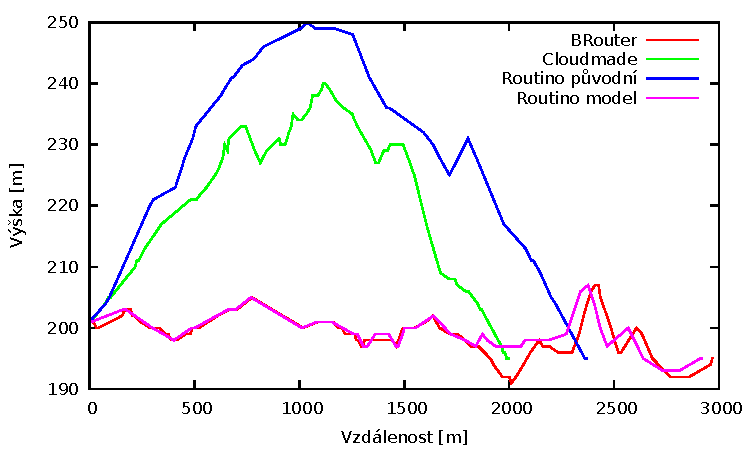
\includegraphics[width=\columnwidth]{porovnani/ele-nus.pdf}
\caption{Nadmořská výška vyhledané trasy dle SRTM z Nuslí do Podolí. }
\label{img:vyska-n}
\end{figure}

\begin{figure}[!ht]
\centering
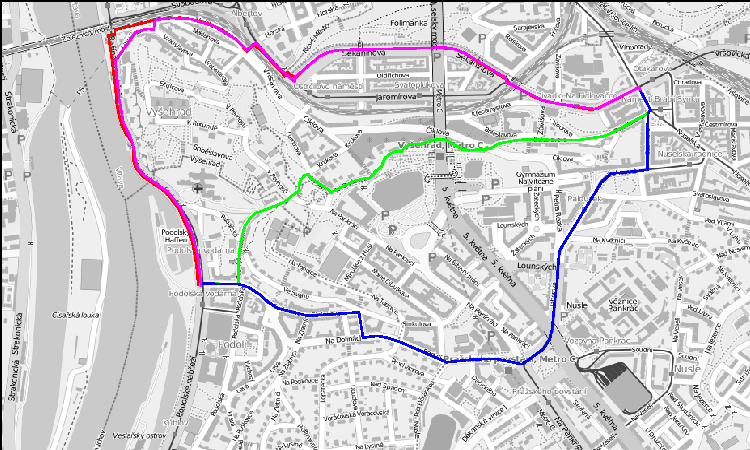
\includegraphics[width=\columnwidth]{porovnani/ll-nus.pdf}
\caption{Zobrazení nad OpenStreetMap podkladem trasy z Nuslí do Podolí. }
\label{img:mapa-n}
\end{figure}














\begin{conclusion}


V~práci jsme se zabývali minimalizací převýšení při vyhledávání tras pro cyklisty. Nejprve jsme ověřili možnosti otevřených dat a porovnali dostupné routovací systémy. Systém Routino vyšel z~porovnání jako nejvhodnější kandidát a implementace zamýšlené vlastnosti se zdařila ve funkční celek.

Abychom získali koeficienty určující rychlosti v~různých klasifikací kopců, připravili jsme analyzér projetých tras, který postavil trasu na digitální zemský model. Posoudili jsme míru rušení GPS záznamu i nepřesnosti dané digitálním modelem.

V~průběhu jsme definovali problém cyklistů jako požadavek na časovou úspornost cesty a implementaci založili na tezi, že cyklistův dojezdový čas je ovlivněn nastoupaným převýšením.

Postupovali jsme podle navrženého modelu z~analyzátoru, ale ve výsledku se ukázalo, že časově vyjde často lépe trasa přes kopec, nežli ta které vede okolo delší vzáleností. Pro cyklistu je tedy žádoucí osobní nastavení a následný výběr z~více možností pro každou naplánovanou trasu.

Ve srovnání vyšlo najevo, že trasa z~routeru opravdu dosahuje minimálních převýšení na zadané trase a může být tak výhodnou alternativou i proti komerčním, běžně používaným systémům.

Do budoucna by se dalo uvažovat o~implementaci nabytých znalostí do pokročilejšího routeru. Routino sice obstojně posloužilo svému účelu, ovšem rozšiřitelnost je díky obsáhlým zdrojovým kódům v~jazyce C velmi náchylná na chyby a ne přilíš pohodlná.


\end{conclusion}











\bibliographystyle{csn690}
\bibliography{mybibliographyfile}


\appendix
\chapter{Seznam použitých zkratek}
% \printglossaries
\begin{description}
	\item[GPS] Global Positioning System -- Globální satelitní navigační systém
	\item[LGPL] Lesser General Public License -- Copyleftová licence, která umožňuje využít práci i v~ne-GPL aplikacích
	\item[AGPL] Affero General Public License -- Copyleftová licence, která vynucuje zpřístupnění odvozených prací i pro síťové uživatele
	\item[BSD] Berkeley Software Distribution -- Licence, která vynucuje pouze zachování jména autora.
	\item[OSM] OpenStreetMap
	\item[XML] Extensible Markup Language
	\item[ŘSD] Ředitelství silnic a dálnic
	\item[CGI] Common Gateway Interface
	\item[API] Application programming interface
	\item[DEM] Digital elevation model 
	\item[SRTM] Shuttle Radar Topography Mission
	\item[ASTER] Advanced Spaceborne Thermal Emission and Reflection
	\item[GPX] GPS eXchange -- Formát vyměny GPS záznamů založený na XML
	
\end{description}


\chapter{Obsah přiloženého CD}

%TODO upravte podle skutecnosti

\begin{figure}
	\dirtree{%
		.1 readme.txt\DTcomment{stručný popis obsahu CD}.
		.1 src.
		.2 instalace.txt\DTcomment{instalační příručka}.		
		.2 routino\DTcomment{zdrojové kódy upraveného routeru}.
		.2 analyzer\DTcomment{zdrojové kódy analyzéru}.
		.3 gpx\DTcomment{uložené záznamy z~GPS}.		
		.3 GeoData\DTcomment{výškový model SRTM -- CGIAR CSI}.				
		.2 srtm-hgt-reader\DTcomment{zdrojové kódy vytvořeného SRTM readeru}.
		.3 srtm\DTcomment{ukázková data SRTM}.		
		.3 aster\DTcomment{ukázková data ASTER GDEM}.				
		.2 thesis\DTcomment{zdrojová forma práce ve formátu \LaTeX{}}.
		.3 grafy\DTcomment{zdrojové soubory v~programu Gnuplot}.		
		.1 text\DTcomment{text práce}.
		.2 thesis.pdf\DTcomment{text práce ve formátu PDF}.
	}
\end{figure}



\chapter{Návod k~instalaci}

Na CD je celý software zkompilován pro architekturu amd64, ale je velice snadné zkompilovat jej pro libovolný systém založený na Linuxu. Kompilátor byl použitý gcc version 4.7.2 na systému Debian Wheezy. 

Upravené soubory jsou verzovány systémem GIT, jehož složka se nachází u~zdrojových kódů routina, analyzéru i srtm-readeru.

\begin{itemize}
\item{Závislosti jsou na knihovnách libzip a libbz2 pro načítání dat. Na systémech Debian, Ubuntu apod. možno nainstalovat přes \\ \verb|apt-get install libzip-dev libbz2-dev|.
}

\item{Kompilace se provádí v~nejvyšší složce \verb|routino| příkazem \verb|make|, ten zároveň i zkopíruje binární programy do složky \verb|web/bin|. 
}

\item{Pro spuštění webového serveru apache2 je nutné nejprve povolit v~globální konfiguraci vhost volbu \verb|AllowOverride All|, následně již je dostupný router přes \verb|http://localhost/routino/web/www/routino/| pakliže fyzicky celou složku umístíme do document rootu.
}

\item{Pro správnou funkci je ještě nutné nastavit správná práva na složku \verb|routino/web/results/|, obvykle postačí \verb|chown www-data results|.}

\end{itemize}




Pro přípravu vlastní routovací databáze možný následující postup:

\begin{itemize}

\item{Stáhnout příslušné dlaždice SRTM dat: \\ \verb|http://dds.cr.usgs.gov/srtm/version2_1/SRTM3/| \\
a vložit je do složky \verb|routino/web/data/srtm|.}

\item{OSM vektorová data možno stáhnout ze serveru \\ \verb|http://download.geofabrik.de|.}

\item{Routovací databázi vytvoříme příkazem \\ 
\verb|routino/web/data$ ../bin/planetsplitter data.osm 2>/dev/null|}

\end{itemize}












\end{document}


